% ChatGPT Directions 0 : 
% This is a Tbox Problem set for the following standards 8.EE.B.5
%--------------------------------------------------
\documentclass[12pt]{article}
\usepackage[a4paper, top=0.8in, bottom=0.7in, left=0.8in, right=0.8in]{geometry}
\usepackage{amsmath}
\usepackage{amsfonts}
\usepackage{latexsym}
\usepackage{graphicx}
\usepackage{fancyhdr}
\usepackage{tcolorbox}
\usepackage{enumitem}
\usepackage{setspace}
\usepackage{tikz}
\usepackage[defaultfam,tabular,lining]{montserrat} % Font settings for Montserrat

% General Comment: Template for creating problem sets in a structured format with headers, titles, and sections.
% This document uses Montserrat font and consistent styles for exercises, problems, and performance tasks.

% -------------------------------------------------------------------

\setlength{\parindent}{0pt}
\pagestyle{fancy}

\setlength{\headheight}{27.11148pt}
\addtolength{\topmargin}{-15.11148pt}

\fancyhf{}
%\fancyhead[L]{\textbf{8.EE.B.5: Graphing and Comparing Proportional Relationships}}
\fancyhead[R]{
\includegraphics[width=0.8cm]{Round Logo.png}} % Placeholder for logo
\fancyfoot[C]{\footnotesize \textcopyright{} Study Smart Tutors}

\sloppy

\title{}
\date{}
\hyphenpenalty=10000
\exhyphenpenalty=10000

\begin{document}

\subsection*{Problem Set: Graphing and Comparing Proportional Relationships}
\onehalfspacing

% Learning Objective Box
\begin{tcolorbox}[colframe=black!40, colback=gray!5, 
coltitle=black, colbacktitle=black!20, fonttitle=\bfseries\Large, 
title=Learning Objective, halign title=center, left=5pt, right=5pt, top=5pt, bottom=15pt]
\textbf{Objective:} Graph proportional relationships, interpret the unit rate as the slope of the graph, and compare proportional relationships represented in different ways.
\end{tcolorbox}

% Exercises Box 1
\begin{tcolorbox}[colframe=black!60, colback=white, 
coltitle=black, colbacktitle=black!15, fonttitle=\bfseries\Large, 
title=Exercises: Unit Rate and Slope, halign title=center, left=10pt, right=10pt, top=10pt, bottom=60pt]
\begin{enumerate}[itemsep=3em]
    \item A car travels \(150 \, \text{miles}\) in \(3 \, \text{hours}\). What is the unit rate of the car's speed? Interpret this as the slope of the proportional relationship.

    \item The graph of a proportional relationship passes through the points \((0, 0)\) and \((6, 18)\). Find the slope of the line and write the equation of the relationship.

    \item A cyclist rides at a constant speed such that the relationship is \(y = 4x\), where \(y\) is the distance (in miles) and \(x\) is the time (in hours). Create a table of values for this relationship and plot the graph on the coordinate plane below.
    
    \begin{center}
        \begin{tikzpicture}[scale=0.8]
            % Draw grid
            \draw[step=1cm, gray!50, thin] (-1,-1) grid (8,8);
            % Draw axes
            \draw[thick, ->] (-1,0) -- (8.5,0) node[right] {\(x\)};
            \draw[thick, ->] (0,-1) -- (0,8.5) node[above] {\(y\)};
            % Label axes
            \foreach \x in {1,2,3,4,5,6,7,8} {
                \draw (\x,0.1) -- (\x,-0.1) node[below] {\(\x\)};
            }
            \foreach \y in {1,2,3,4,5,6,7,8} {
                \draw (0.1,\y) -- (-0.1,\y) node[left] {\(\y\)};
            }

\draw (-.4,-.1) node[below] {$O$};


\draw (-1,5) node[left] {\textit \textbf{Miles}};

  \draw (5,-2) node[left] {\textit\textbf{Hours}};          
        \end{tikzpicture}
    \end{center}
\end{enumerate}
\end{tcolorbox}

% Exercises Box 2
\begin{tcolorbox}[colframe=black!60, colback=white, 
coltitle=black, colbacktitle=black!15, fonttitle=\bfseries\Large, 
title=Exercises: Graphing and Comparison, halign title=center, left=10pt, right=10pt, top=10pt, bottom=60pt]
\begin{enumerate}[itemsep=3em, start=4]
    \item Compare the following proportional relationships:
    \begin{itemize}
        \item A worker earns \$72 after \(6 \, \text{hours of work}\).
        \item A worker earns \$120 after \(10 \, \text{hours of work}\).
    \end{itemize}
    Write the equations for both relationships, graph them on the same coordinate plane below, and explain which worker earns more per hour.

    \begin{center}
        \begin{tikzpicture}[scale=0.8]
            % Draw grid
            \draw[step=1cm, gray!50, thin] (-1,-1) grid (12,12);
            % Draw axes
            \draw[thick, ->] (-1,0) -- (12.5,0) node[right] {\(x\)};
            \draw[thick, ->] (0,-1) -- (0,12.5) node[above] {\(y\)};
            % Label axes
            \foreach \x in {0,2,4,6,8,10,12} {
                \draw (\x,0.2) -- (\x,-0.2) node[below] {\(\x\)};
            }
            \foreach \y in {0,2,4,6,8,10,12} {
                \draw (0.2,\y) -- (-0.2,\y) node[left] {\(\y\)};
            }
        \end{tikzpicture}
    \end{center}

    \item Graph the proportional relationship \(y = 5x\) on the coordinate plane below. Label the slope and provide two additional points on the graph.

    \begin{center}
        \begin{tikzpicture}[scale=0.8]
            % Draw grid
            \draw[step=1cm, gray!50, thin] (-1,-1) grid (8,8);
            % Draw axes
            \draw[thick, ->] (-1,0) -- (8.5,0) node[right] {\(x\)};
            \draw[thick, ->] (0,-1) -- (0,8.5) node[above] {\(y\)};
            % Label axes
            \foreach \x in {0,1,2,3,4,5,6,7,8} {
                \draw (\x,0.1) -- (\x,-0.1) node[below] {\(\x\)};
            }
            \foreach \y in {0,1,2,3,4,5,6,7,8} {
                \draw (0.1,\y) -- (-0.1,\y) node[left] {\(\y\)};
            }
        \end{tikzpicture}
    \end{center}
\end{enumerate}
\end{tcolorbox}


\vspace{1em}

% Problems Box
\begin{tcolorbox}[colframe=black!60, colback=white, 
coltitle=black, colbacktitle=black!15, fonttitle=\bfseries\Large, 
title=Problems, halign title=center, left=10pt, right=10pt, top=10pt, bottom=60pt]
\begin{enumerate}[start=6, itemsep=3em]
    \item Compare the following proportional relationships:
    \begin{itemize}
        \item A graph shows a line passing through \((0, 0)\) and \((2, 10)\).
        \item A table shows:
        \begin{tabular}{|c|c|}
        \hline
        \(x\) & \(y\) \\
        \hline
        0 & 0 \\
        1 & 6 \\
        2 & 12 \\
        \hline
        \end{tabular}
    \end{itemize}
    Which relationship has the greater unit rate? Explain.
    \item A distance-time graph shows a car traveling at a constant speed of 60 miles per hour. Another car's equation is given as \(y = 45x\). Compare the speeds of the two cars and determine which one is faster.
    \item A water hose fills a pool at a rate of 4 gallons per minute. Graph this relationship and interpret the slope.
    \item Two runners are jogging at constant speeds:
    \begin{itemize}
        \item Runner A: A graph passes through \((0, 0)\) and \((1, 8)\).
        \item Runner B: A table shows:
        \begin{tabular}{|c|c|}
        \hline
        \(x\) & \(y\) \\
        \hline
        0 & 0 \\
        1 & 10 \\
        2 & 20 \\
        \hline
        \end{tabular}
    \end{itemize}
    Which runner is faster? Justify your answer.
\end{enumerate}
\end{tcolorbox}

\vspace{1em}

% Performance Task Box
\begin{tcolorbox}[colframe=black!60, colback=white, 
coltitle=black, colbacktitle=black!15, fonttitle=\bfseries\Large, 
title=Performance Task: Comparing Travel Speeds, halign title=center, left=10pt, right=10pt, top=10pt, bottom=50pt]
\textbf{Scenario:} Two cyclists are biking on flat roads:
\begin{itemize}
    \item Cyclist A's graph passes through \((0, 0)\) and \((2, 20)\).
    \item Cyclist B's equation is \(y = 15x\).
\end{itemize}
\textbf{Task:}
\begin{enumerate}[itemsep=3em]
    \item Compare the unit rates (slopes) for Cyclist A and Cyclist B.
    \item Determine who is biking faster. Justify your answer.
    \item Graph both relationships on the same coordinate plane.
    \item Create a real-world scenario where understanding the unit rate is essential and explain its importance.
\end{enumerate}
\end{tcolorbox}

\vspace{1em}

% Reflection Box
\begin{tcolorbox}[colframe=black!60, colback=white, 
coltitle=black, colbacktitle=black!15, fonttitle=\bfseries\Large, 
title=Reflection, halign title=center, left=10pt, right=10pt, top=10pt, bottom=80pt]
Reflect on how proportional relationships and slopes help in solving real-world problems. Why is the y-intercept always \(0\) in proportional relationships? Provide an example where interpreting a graph of a proportional relationship is useful.
\end{tcolorbox}

\end{document}
